\documentclass[11pt]{article}

\usepackage[a4paper,margin=2.5cm]{geometry}
\usepackage{fontspec}
\usepackage{titlesec}
\usepackage{xcolor}
\usepackage{tcolorbox}
\usepackage{booktabs}
\usepackage{longtable}
\usepackage{array}
\usepackage{enumitem}
\usepackage{hyperref}
\usepackage{listings}
\usepackage{parskip}
\usepackage{fancyhdr}
\usepackage{graphicx}

\definecolor{navy}{HTML}{1B3A57}
\definecolor{codebg}{HTML}{F5F5F0}
\definecolor{bugred}{HTML}{9B2C2C}
\definecolor{fixgreen}{HTML}{276749}

\titleformat{\section}{\large\bfseries\color{navy}}{\thesection}{0.6em}{}
\titleformat{\subsection}{\normalsize\bfseries\color{navy}}{\thesubsection}{0.6em}{}

\hypersetup{
  colorlinks=true,
  linkcolor=navy,
  urlcolor=navy,
  citecolor=navy,
  pdftitle={Agentic SOC Assistant --- Architecture Evaluation and Research Roadmap},
  pdfauthor={Internship Project}
}

\lstdefinestyle{code}{
  backgroundcolor=\color{codebg},
  basicstyle=\ttfamily\small,
  breaklines=true,
  frame=single,
  rulecolor=\color{gray!40},
  columns=fullflexible,
  showstringspaces=false
}
\lstset{style=code}

\pagestyle{fancy}
\fancyhf{}
\fancyhead[L]{\small\color{gray} Agentic SOC Assistant --- Architecture Report}
\fancyhead[R]{\small\color{gray} \thepage}
\renewcommand{\headrulewidth}{0.3pt}

\newenvironment{bugbox}[1]{%
  \begin{tcolorbox}[colback=bugred!5,colframe=bugred!70!black,title=\textbf{#1},fonttitle=\bfseries,boxrule=0.6pt]
}{\end{tcolorbox}}

\newenvironment{fixbox}[1]{%
  \begin{tcolorbox}[colback=fixgreen!5,colframe=fixgreen!60!black,title=\textbf{#1},fonttitle=\bfseries,boxrule=0.6pt]
}{\end{tcolorbox}}

\title{\color{navy}\textbf{Agentic SOC Assistant}\\[0.3em]
\large Architecture Evaluation, Bug Audit, Demo Roadmap,\\ Research Improvements, and Benchmarking Protocol}
\author{Internship Research Project --- Multi-Agent AI for SOC Alert Triage}
\date{\today}

\begin{document}
\maketitle

\begin{abstract}
\noindent This report evaluates the \emph{Agentic SOC Assistant} repository against its intended architecture (LangGraph orchestrator, four specialist agents, a reasoning-synthesis stage, a structurally-enforced human-in-the-loop boundary, and a four-store RAG knowledge base). It is organized into five parts, matching the project's research framing as \emph{``a proof of concept to validate the research direction rather than being only an engineering deliverable''}: (1) an evaluation of the current architecture and implementation; (2) a concrete list of bugs and gaps found in the code; (3) a phased, actionable plan to reach a working end-to-end demo; (4) research-oriented improvements to the multi-agent design, each grounded in a specific reference; and (5) a benchmarking protocol suitable for the stated evaluation axes (triage accuracy, report quality, time reduction, explainability, false-positive handling, and MITRE ATT\&CK alignment). Section~\ref{sec:integration} documents the modifications made directly in the repository alongside this report.
\end{abstract}

\tableofcontents

% ======================================================================
\section{System Overview}
\label{sec:overview}

The target architecture (Figure~\ref{fig:diagram}, reproduced from the project's design diagram) is a six-stage LangGraph pipeline sitting behind a hard human-in-the-loop (HITL) boundary:

\begin{figure}[h]
\centering
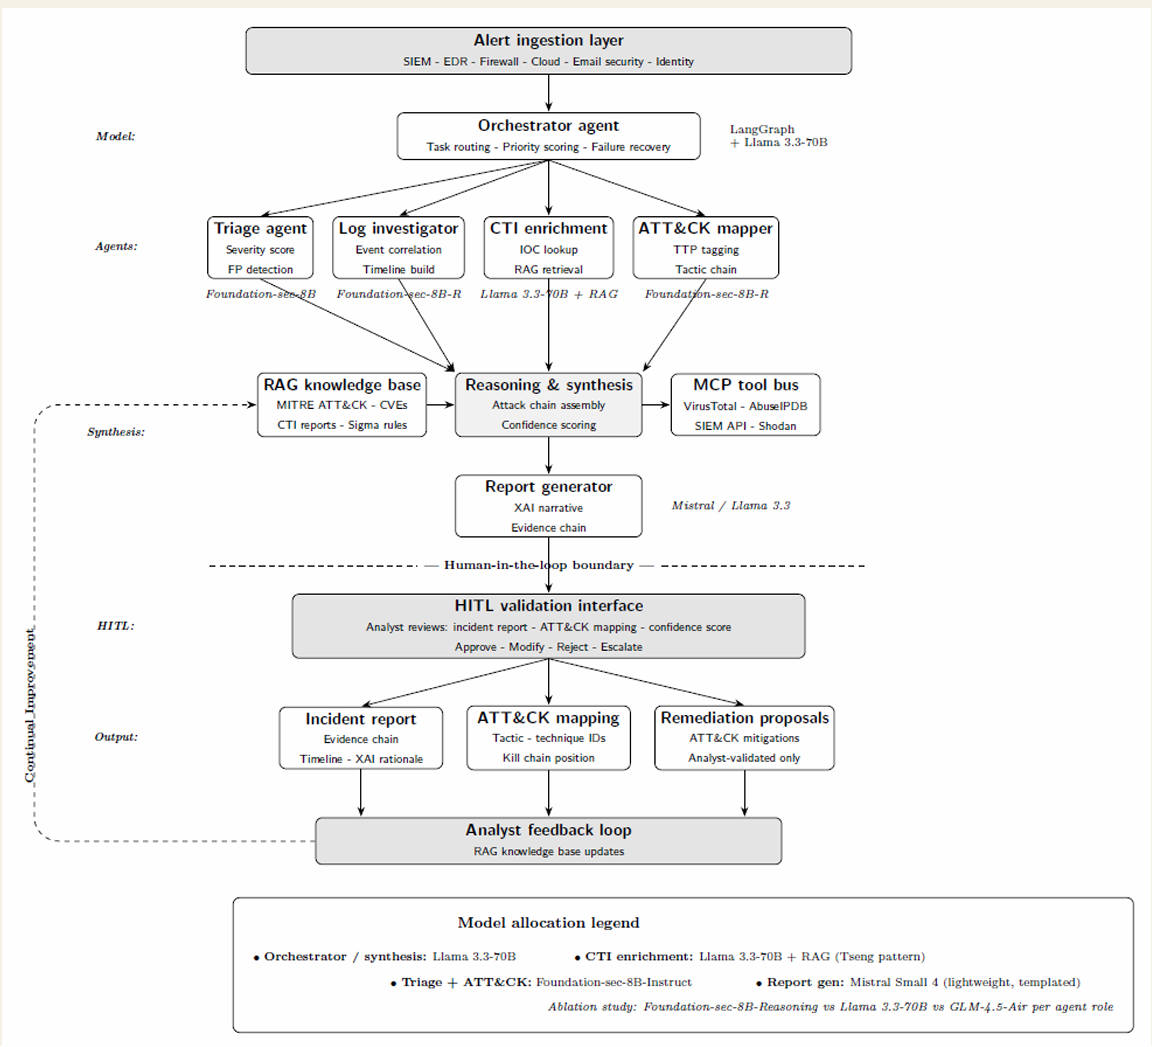
\includegraphics[width=0.92\textwidth]{architecture_diagram.png}
\caption{Target architecture: alert ingestion, LangGraph orchestrator, four parallel specialist agents, reasoning \& synthesis, report generation, the HITL boundary, and the analyst feedback loop back into the RAG knowledge base.}
\label{fig:diagram}
\end{figure}

\begin{enumerate}[label=\arabic*.]
  \item \textbf{Alert ingestion layer} --- SIEM, EDR, Firewall, Cloud, Email security, Identity sources normalized into a single schema.
  \item \textbf{Orchestrator agent} --- task routing, priority scoring, failure recovery, implemented as a LangGraph \texttt{StateGraph}.
  \item \textbf{Four parallelizable specialist agents} --- Triage, Log Investigator, CTI Enrichment, ATT\&CK Mapper.
  \item \textbf{Reasoning \& synthesis} --- attack-chain assembly and confidence scoring over the four agents' typed outputs.
  \item \textbf{Report generator} --- an explainable (XAI) narrative plus evidence chain.
  \item \textbf{HITL validation interface} --- analyst approve/modify/reject/escalate, the \emph{only} path that can authorize remediation, feeding an analyst feedback loop back into the RAG knowledge base.
\end{enumerate}

\begin{table}[h]
\centering
\small
\begin{tabular}{@{}ll@{}}
\toprule
\textbf{Diagram component} & \textbf{Repository location} \\
\midrule
Orchestrator agent & \texttt{soc-assistant/orchestrator/graph.py} \\
Triage / Log Investigator / CTI / ATT\&CK & \texttt{soc-assistant/agents/*.py} \\
Reasoning \& synthesis & \texttt{soc-assistant/agents/synthesis.py}, \texttt{models/synthesis.py} \\
Report generator & \texttt{soc-assistant/agents/report\_generator.py} \\
RAG knowledge base (4 stores) & \texttt{soc-assistant/rag/store\_*.py}, \texttt{rag/indexer.py} \\
MCP tool bus (read-only / RAG / write) & \texttt{soc-assistant/mcp\_tools/\{read\_only,rag,write\}/api.py} \\
HITL validation interface & \texttt{soc-assistant/hitl/api.py} \\
Analyst feedback loop & \texttt{soc-assistant/review/feedback/rag\_update.py} \\
Shared pipeline state & \texttt{soc-assistant/state/investigation.py} \\
Model allocation legend & \texttt{soc-assistant/config/models.yaml} (updated, \S\ref{sec:integration}) \\
\bottomrule
\end{tabular}
\caption{Mapping between the architecture diagram and the current repository layout.}
\end{table}

% ======================================================================
\section{Part 1 --- Architecture and Implementation Evaluation}
\label{sec:eval}

\subsection{What is solid}

\begin{itemize}
  \item \textbf{Typed contracts everywhere.} \texttt{schemas/alert.py}, \texttt{schemas/agent\_io.py}, and \texttt{models/synthesis.py} give every agent boundary a Pydantic model. This is exactly what the spec asked for (``never free text between agents'') and it is already load-bearing: the orchestrator, the agents, and the report generator all read/write through these types rather than ad hoc dicts.
  \item \textbf{The safety boundary is structural, not prompted.} \texttt{mcp\_tools/write/api.py} raises an HTTP 403 if \texttt{approved\_by} is empty, for all four write tools (\texttt{isolateHost}, \texttt{disableUserAccount}, \texttt{blockIPFirewall}, \texttt{createTicket}). Combined with \texttt{state/investigation.py} keeping \texttt{approved\_by} as a dedicated field only the HITL endpoint is supposed to populate, this is a genuine enforcement mechanism, not a policy documented in a prompt that an agent could talk its way around.
  \item \textbf{The orchestrator graph correctly encodes the conditional/parallel/failure-recovery requirements at the code level.} \texttt{route\_after\_triage} skips the log investigator for \texttt{impossible\_travel} alerts, the three specialist nodes are wired as independent edges converging into \texttt{reasoning\_synthesis}, and \texttt{retry\_wrapper} implements the retry-then-degrade-gracefully pattern (append to \texttt{missing\_evidence} rather than crash).
  \item \textbf{The escalation policy is enforced as code, not left to model discretion.} \texttt{agents/synthesis.py} already branches on the confidence thresholds from \texttt{config/thresholds.yaml} and forces escalation whenever \texttt{remediation\_required} is true, matching the spec's explicit table.
  \item \textbf{The RAG store design correctly differentiates retrieval methods per store}: Chroma vector stores for ATT\&CK/CTI (semantic, unstructured text), raw SQLite key-value for IOCs and the org knowledge base (exact-match, no embedding needed). This is the right call --- embedding an IP address or a hostname buys nothing over an indexed lookup.
\end{itemize}

\subsection{What is missing or shallow}

\begin{itemize}
  \item \textbf{No agent currently calls a model or a tool.} Every function in \texttt{agents/*.py} returns a hardcoded placeholder (e.g. triage always emits severity 7.5). The pipeline topology, typing, and safety boundary are real; the actual cognitive work the research question is about --- ``how AI agents improve efficiency, explainability, reliability'' --- has not been implemented yet. This is the single largest gap between architecture and implementation.
  \item \textbf{MCP is a naming convention, not a protocol, today.} \texttt{mcp\_tools/read\_only/api.py} and \texttt{mcp\_tools/rag/api.py} are plain Python functions (\texttt{pass}); nothing in the repo runs an actual MCP server or exposes these as MCP tool schemas. The one part of the MCP boundary that \emph{is} meaningfully implemented is the write-tool approval gate --- but even that is a plain function you would call directly, not something reachable only through an MCP transport. As written, an agent \emph{could} still call \texttt{isolateHost} directly in-process without going through any protocol boundary; the only thing stopping it is the \texttt{approved\_by} check inside the function body itself, which is good practice but does not yet match ``the MCP server must reject any call missing a valid \texttt{approved\_by} field'' as an infrastructure guarantee.
  \item \textbf{The orchestrator is deterministic control flow, while the diagram implies an LLM-driven orchestrator} (``Orchestrator agent --- LangGraph + Llama 3.3-70B''). There is a real design decision to make here (\S\ref{sec:bugs}, item~7): keep routing deterministic (auditable, reproducible, cheap) and reserve the LLM for \emph{priority scoring} only, or actually let the orchestrator's own reasoning influence routing. For a safety-sensitive SOC system, the former is almost certainly the right call, but it is worth stating explicitly rather than leaving it implicit.
  \item \textbf{No real evaluation data exists yet.} \texttt{data/alerts/} and \texttt{data/logs/} are empty except for \texttt{.gitkeep}; \texttt{tests/} contains only an \texttt{\_\_init\_\_.py}. There is no fixture alert, no seed ATT\&CK/CTI content actually indexed (the indexer exists but has not been run), and no test asserting that the graph executes end to end.
  \item \textbf{HITL endpoints are unwired.} \texttt{hitl/api.py} returns hardcoded empty payloads; nothing reads from the LangGraph \texttt{SqliteSaver} checkpoint, nothing forwards an approved decision to the write MCP tools, and nothing calls \texttt{review/feedback/rag\_update.py} on modify/reject. The API \emph{shape} is correct; the \emph{behavior} is not implemented.
  \item \textbf{The feedback loop and per-role evaluation are stubs.} \texttt{review/feedback/rag\_update.py} is a no-op; \texttt{eval/override\_rate.py} originally computed one pipeline-wide ratio rather than the per-agent-role breakdown the spec explicitly asks for (fixed in \S\ref{sec:integration}).
\end{itemize}

\subsection{Overall assessment}

The repository is best described as \textbf{a correctly-typed, correctly-orchestrated skeleton with the safety boundary already in the right place, and all of the actual intelligence still to be added.} That is a defensible state for a research-oriented internship at this stage: the architecture decisions that are hard to walk back later (state shape, the HITL gate, the escalation-policy-as-code pattern) are already committed to code rather than left as prose, which is exactly the kind of thing that makes a later paper's methodology section credible. The risk is scope: the remaining work (real model calls, real MCP transport, real RAG content, real HITL wiring, and only then evaluation) is substantial and should be planned explicitly (\S\ref{sec:demo}) rather than assumed to be incremental.

% ======================================================================
\section{Part 2 --- Problems and Bugs}
\label{sec:bugs}

\begin{bugbox}{Bug 1 --- Broken import in \texttt{rag/indexer.py}}
\texttt{indexer.py} originally imported \texttt{from .stores import attck\_store}, but no \texttt{stores.py} module exists in \texttt{rag/} --- the vector store is defined in \texttt{store\_attck.py}. Running the indexer as-is raises \texttt{ModuleNotFoundError} immediately. \textit{Status: fixed in this pass, see \S\ref{sec:integration}.}
\end{bugbox}

\begin{bugbox}{Bug 2 --- \texttt{model\_id} defaults contradict the architecture diagram}
\texttt{config/models.yaml} originally pointed every agent role at a single hosted \texttt{grok-4-fast} model (the build prompt's documented fallback path), while the architecture diagram specifies a per-role allocation across Foundation-Sec-8B variants, Llama~3.3-70B, and Mistral Small. These are not in conflict as \emph{options} (the build prompt explicitly designs for this as a config-only toggle), but leaving the file in its fallback state while treating the diagram as ``the'' architecture is misleading --- anyone reading \texttt{models.yaml} today would conclude the project runs entirely on one hosted model with no differentiation. \textit{Status: fixed in this pass; \texttt{models.yaml} now encodes the diagram's allocation as primary with the Grok fallback documented per role, see \S\ref{sec:integration}.}
\end{bugbox}

\begin{bugbox}{Bug 3 --- Internal inconsistency inside the diagram itself}
The diagram's per-box labels give the Log Investigator and ATT\&CK Mapper \texttt{Foundation-sec-8B-R} (Reasoning variant), while the legend's summary line groups ``Triage + ATT\&CK: Foundation-sec-8B-Instruct'' and does not mention the Log Investigator at all. As implemented in this pass, Triage uses the Instruct variant (fast classification) and both Log Investigator and ATT\&CK Mapper use the Reasoning variant (multi-step correlation), following the per-box labels rather than the legend's shorthand --- but this should be confirmed against whatever internal design conversation produced the diagram, since it changes cost and latency assumptions per role.
\end{bugbox}

\begin{bugbox}{Bug 4 --- \texttt{SqliteSaver.from\_conn\_string} usage may not match the installed \texttt{langgraph-checkpoint-sqlite} API}
Recent versions of \texttt{langgraph-checkpoint-sqlite} require \texttt{SqliteSaver.from\_conn\_string(...)} to be used as a context manager (\texttt{with SqliteSaver.from\_conn\_string(...) as saver:}) rather than assigned directly, because the underlying sqlite3 connection needs a lifecycle. \texttt{orchestrator/graph.py} assigns it directly to \texttt{checkpointer}. This may raise at import/build time depending on the exact pinned version; \texttt{requirements.txt} does not pin an exact version (\texttt{>=1.0.0}), so this should be verified against whatever version actually resolves.
\end{bugbox}

\begin{bugbox}{Bug 5 --- CRLF line endings in YAML configs}
All three files under \texttt{config/} were saved with Windows-style \texttt{\textbackslash r\textbackslash n} line endings. PyYAML tolerates this, but it is a needless source of noisy diffs and potential friction if the project is ever edited on a mixed Windows/Linux team or picked up by tooling that is stricter about line endings. \textit{Status: normalized to LF in this pass, see \S\ref{sec:integration}.}
\end{bugbox}

\begin{bugbox}{Bug 6 --- \texttt{eval/override\_rate.py} does not attribute overrides per agent role}
The spec explicitly asks to ``attribute each modification to which upstream agent's output was corrected, not just a single pipeline-wide number,'' but the original implementation only computed one flat ratio. \textit{Status: \texttt{calculate\_override\_rate\_by\_role} added in this pass, see \S\ref{sec:integration}.}
\end{bugbox}

\begin{bugbox}{Bug 7 (design ambiguity, not a code bug) --- Orchestrator's LLM role is undefined}
The diagram labels the orchestrator ``LangGraph + Llama 3.3-70B,'' implying the orchestrator itself makes an LLM call for ``task routing, priority scoring.'' The current \texttt{orchestrator/graph.py} implements routing as pure deterministic Python (threshold comparisons on \texttt{severity}/\texttt{category}). Nothing in the code shows where or how the Llama~3.3-70B call for ``priority scoring'' would plug in. This needs an explicit decision (recommendation: keep \emph{routing} deterministic for auditability, and add a narrow, separately-logged LLM call that only produces a \emph{priority score} annotation consumed by, but not overriding, the deterministic router).
\end{bugbox}

\begin{bugbox}{Bug 8 --- \texttt{models/synthesis.py} lives outside \texttt{schemas/}}
Every other typed I/O contract lives under \texttt{schemas/}; \texttt{SynthesisOutput} alone lives under a sibling \texttt{models/} directory with no other content. Not a functional bug, but worth normalizing (either move it into \texttt{schemas/synthesis.py}, or move all Pydantic models into \texttt{models/} and rename \texttt{schemas/} accordingly) before the codebase grows further.
\end{bugbox}

\begin{bugbox}{Bug 9 --- No test coverage}
\texttt{tests/} contains only an empty \texttt{\_\_init\_\_.py}. There is currently no automated check that the graph compiles, that \texttt{route\_after\_triage} returns the expected node set for each category, or that the write-tool approval gate actually rejects an unapproved call. Given this project's stated safety framing, at minimum the approval-gate rejection path deserves a regression test before any real agent logic is added on top.
\end{bugbox}

% ======================================================================
\section{Part 3 --- Structured Path to a Running Demo}
\label{sec:demo}

The phases below are ordered by dependency, not by estimated effort; each phase should produce something runnable before moving to the next, so that a partial demo always exists.

\begin{enumerate}[label=\textbf{Phase \arabic*:}, leftmargin=2.2cm, itemsep=0.6em]

\item \textbf{Fix the known bugs (\S\ref{sec:bugs}).} Apply Bugs 1, 2, 5, 6 (already applied in this pass, \S\ref{sec:integration}); resolve the \texttt{SqliteSaver} context-manager question (Bug 4) by pinning an exact \texttt{langgraph-checkpoint-sqlite} version and testing graph compilation in isolation; make an explicit decision on Bug 7 (orchestrator LLM role) and document it in \texttt{docs/ARCHITECTURE.md}.

\item \textbf{Stand up one model endpoint end-to-end before wiring all six roles.} Pick the cheapest path to a working call: either the documented Grok fallback (zero infra, immediate) or a single self-hosted \texttt{vLLM}/\texttt{Ollama} endpoint serving one Foundation-Sec-8B variant. Get one agent (Triage is the simplest --- four read-only tools, no RAG dependency) actually calling a real model and returning a real \texttt{TriageOutput}, with a unit test asserting the output validates against the schema.

\item \textbf{Implement the MCP transport, not just the approval-gate function.} Use the official \texttt{mcp} Python SDK (or \texttt{FastMCP}) to expose \texttt{read\_only}, \texttt{rag}, and \texttt{write} as three separate MCP servers/namespaces, matching the spec's ``separate MCP servers or separate namespaces, not just a naming convention.'' Keep the existing \texttt{validate\_approval} logic, but move the enforcement point to the MCP server's tool-call handler so an agent process literally cannot reach \texttt{isolateHost} without going through the protocol layer.

\item \textbf{Populate the RAG stores with real seed data.} Run (the now-fixed) \texttt{rag/indexer.py} to index the MITRE ATT\&CK STIX bundle into Store~1. Seed Store~2 (CTI reports) with a handful of public Mandiant/CISA/Unit42 blog posts or advisories relevant to a small number of techniques you intend to demo against. Populate Store~3 (IOC) and Store~4 (org KB) with a synthetic org: a handful of fake hosts/users/assets and a few known-malicious/known-benign IPs, enough to make \texttt{checkMaintenanceWindow} and \texttt{exclusivity} scoring meaningfully testable.

\item \textbf{Implement the remaining five agents against real read-only/RAG tools.} Log Investigator and CTI Enrichment first (they are the parallel branch the spec emphasizes), then ATT\&CK Mapper (depends on Store~1 fusion), then Reasoning \& Synthesis (depends on all four upstream outputs), then Report Generator last.

\item \textbf{Build the alert generator / source adapters as mocks, not real connectors.} Per the spec, the six source adapters are explicitly out of scope for real implementation in this pass --- write a small generator that emits \texttt{NormalizedAlert} instances mimicking each source type (including at least one \texttt{impossible\_travel} identity alert to exercise conditional routing, and one high-severity/high-confidence alert to exercise the fast-path side-channel).

\item \textbf{Wire the HITL FastAPI endpoints to the actual LangGraph checkpoint.} \texttt{GET /investigations/\{id\}} should read the persisted \texttt{SOCInvestigationState} from the \texttt{SqliteSaver} checkpoint and return evidence \emph{before} \texttt{synthesis\_output}, per the spec's ordering requirement. \texttt{POST /investigations/\{id\}/decision} should be the only code path that sets \texttt{approved\_by} and forwards remediation to the write MCP server.

\item \textbf{Wire the feedback loop.} On \texttt{modify}/\texttt{reject}, \texttt{review/feedback/rag\_update.py} should actually re-embed the corrected verdict into the relevant store, and the HITL decision handler should pass \texttt{corrected\_fields} in the shape expected by the now-implemented \texttt{eval/override\_rate.py:calculate\_override\_rate\_by\_role} (\S\ref{sec:integration}).

\item \textbf{Add a minimal demo harness.} A CLI script or Jupyter notebook that: generates a batch of mock alerts $\rightarrow$ runs each through \texttt{build\_soc\_graph()} $\rightarrow$ prints the report + confidence + escalation flag $\rightarrow$ optionally pauses for a mock HITL decision via stdin. This does not require the analyst frontend (explicitly out of scope) --- it only needs to prove the graph runs end to end against real (if minimal) data.

\item \textbf{Only then, evaluate.} Section~\ref{sec:benchmark} assumes Phases 1--9 are complete; running an evaluation against a system with hardcoded stub outputs will produce numbers that do not mean anything.

\end{enumerate}

\begin{fixbox}{Milestone definition of ``done'' for the demo}
A single command runs a batch of $\geq$10 synthetic alerts (including at least one identity-only, one high-severity fast-path, and one deliberately noisy/false-positive-prone alert) through the full graph, produces a report with a real (not hardcoded) confidence score and narrative for each, and at least one alert reaches the HITL endpoint where a mock ``modify'' decision visibly changes the override-rate counter for the corrected agent role.
\end{fixbox}

% ======================================================================
\section{Part 4 --- Research-Oriented Improvements}
\label{sec:improvements}

These are framed against the research question stated in the project description: \emph{how AI agents can improve the efficiency, explainability, and reliability of SOC workflows while reducing analyst workload and maintaining safe decision-making.} Each improvement below is scoped to one part of that question and points to a specific reference to read before implementing it, rather than being a generic agent-framework wishlist.

\subsection{Reliability: reduce single-pass hallucination in triage and ATT\&CK mapping}
Route the triage and ATT\&CK-mapping outputs through a lightweight multi-agent debate or self-consistency step before they enter synthesis, rather than trusting one forward pass. Sampling $k$ independent reasoning traces and taking a majority/consistency vote is cheap or free with a fast model like Foundation-Sec-8B-Instruct, and the multi-agent debate framing generalizes naturally to a setting where you already have several distinct agents disagreeing over the same alert. \textbf{Read:} Wang et al., \emph{Self-Consistency Improves Chain of Thought Reasoning in Language Models}, arXiv:2203.11171 (2022); Du et al., \emph{Improving Factuality and Reasoning in Language Models through Multiagent Debate}, arXiv:2305.14325 (2023).

\subsection{Reliability: give the reasoning-synthesis agent an explicit self-correction pass}
Rather than emitting the synthesis verdict in a single forward pass, add a critique-and-revise loop: the synthesis agent first drafts a verdict, then a second (cheap) pass explicitly checks the draft against the \texttt{missing\_evidence} flags and any contradictory upstream signals (e.g. low triage severity plus high-confidence CTI attribution --- already flagged as a case to reconcile in \texttt{agents/synthesis.py}), and only then finalizes. This directly operationalizes the spec's ``reconcile contradictory signals --- weight, don't concatenate'' requirement. \textbf{Read:} Madaan et al., \emph{Self-Refine: Iterative Refinement with Self-Feedback}, arXiv:2303.17651 (2023); Shinn et al., \emph{Reflexion: Language Agents with Verbal Reinforcement Learning}, arXiv:2303.11366 (2023).

\subsection{Explainability: check whether the synthesis narrative actually reflects the confidence score it reports}
A known failure mode in chain-of-thought-style explanations is that the stated rationale does not faithfully reflect the actual decision process (the model reports a plausible-sounding reason after the fact rather than the reason it actually used). This matters directly for the report generator's ``XAI narrative,'' since an analyst reviewing the evidence chain is trusting the narrative to be a genuine explanation, not a post-hoc rationalization. Building a lightweight faithfulness check (e.g. perturbing one piece of upstream evidence and checking whether the narrative and confidence score change accordingly) would be a genuinely novel evaluation axis for a SOC-specific paper. \textbf{Read:} Turpin et al., \emph{Language Models Don't Always Say What They Think: Unfaithful Explanations in Chain-of-Thought Prompting}, arXiv:2305.04388 (2023).

\subsection{Reliability: calibrate confidence scores instead of trusting the model's stated number}
\texttt{agents/synthesis.py}'s escalation policy is only as good as the confidence number feeding it; an LLM's self-reported confidence is well known to be poorly calibrated (over- or under-confident relative to actual correctness). Two complementary directions worth reading before choosing one: (a) probing whether the model's internal representations already ``know'' when it is wrong, which can inform a lightweight calibration head; (b) wrapping the escalation thresholds in a conformal-prediction procedure, which gives a distribution-free statistical guarantee on the escalation policy's error rate rather than an ad hoc 0.65/0.80 cutoff. \textbf{Read:} Kadavath et al., \emph{Language Models (Mostly) Know What They Know}, arXiv:2207.05221 (2022); Angelopoulos and Bates, \emph{A Gentle Introduction to Conformal Prediction and Distribution-Free Uncertainty Quantification}, arXiv:2107.07511 (2021); Quach et al., \emph{Conformal Language Modeling}, arXiv:2306.10193 (2023).

\subsection{Efficiency: fuse Store~1/Store~2 retrieval with a graph-aware method instead of flat RRF alone}
The spec calls for reciprocal rank fusion (RRF) across dense/sparse retrieval for the ATT\&CK and CTI stores, which is a solid baseline. A stronger direction for the ATT\&CK-mapping specifically is to exploit the fact that MITRE ATT\&CK is itself a graph (tactics $\to$ techniques $\to$ sub-techniques $\to$ groups), which flat chunk-based RAG discards. A graph-aware retrieval layer over Store~1 would let the ATT\&CK mapper answer ``what technique plausibly follows this one in a kill chain'' (the \texttt{predicted\_next} field already in \texttt{ATTCKMapperOutput}) far more directly than re-deriving kill-chain adjacency from flat text chunks each time. \textbf{Read:} Cormack, Clarke, and Buettcher, \emph{Reciprocal Rank Fusion Outperforms Condorcet and Individual Rank Learning Methods}, SIGIR 2009 (for the RRF baseline already specified); Edge et al., \emph{From Local to Global: A Graph RAG Approach to Query-Focused Summarization}, arXiv:2404.16130 (2024) (for the graph-aware upgrade).

\subsection{Efficiency: route cheaper models to cheaper decisions instead of a fixed per-role assignment}
The architecture diagram already assigns different model sizes per role (8B for triage/ATT\&CK, 70B for orchestrator/synthesis/CTI), which is directionally the right idea, but it is a static assignment. A cascading/routing approach that only escalates a given alert to the larger model when the smaller model's confidence is low would cut cost and latency further, and gives you a natural research axis (cost vs. accuracy trade-off curve) for the eventual paper. \textbf{Read:} Chen, Zaharia, and Zou, \emph{FrugalGPT: How to Use Large Language Models While Reducing Cost and Improving Performance}, arXiv:2305.05176 (2023); Wang et al., \emph{Mixture-of-Agents Enhances Large Language Model Capabilities}, arXiv:2406.04692 (2024).

\subsection{Reliability: make tool use itself more robust, not just the reasoning around it}
Once the MCP transport is real (\S\ref{sec:demo}, Phase~3), the actual failure mode to worry about shifts from ``does the agent reason correctly'' to ``does the agent call the right tool with the right arguments, and recover sensibly when a tool call fails or returns unexpected data.'' The retry-then-degrade pattern already in \texttt{orchestrator/graph.py} handles \emph{node}-level failure; it is worth separately testing \emph{tool-call}-level failure (e.g. a malformed IOC lookup response) using the same interleaved reasoning/acting pattern the field has converged on. \textbf{Read:} Yao et al., \emph{ReAct: Synergizing Reasoning and Acting in Language Models}, arXiv:2210.03629 (2022); Schick et al., \emph{Toolformer: Language Models Can Teach Themselves to Use Tools}, arXiv:2302.04761 (2023).

\subsection{Domain grounding: verify the security-specific model choice against its own published benchmarks}
Before committing the triage/log-investigator/ATT\&CK roles to Foundation-Sec-8B variants, it is worth reading the model's own technical reports rather than assuming domain-tuning transfers automatically to \emph{this} pipeline's specific tasks (severity scoring, parent-process anomaly flagging, technique classification) --- these are related to but not identical to the benchmarks the model was evaluated on. \textbf{Read:} Kassianik et al., \emph{Llama-3.1-FoundationAI-SecurityLLM-Base-8B Technical Report}, arXiv:2504.21039 (2025) (base model); the companion Foundation-Sec-8B-Instruct technical report, arXiv:2508.01059 (2025) (instruction-tuned variant used for chat-style agent roles).

% ======================================================================
\section{Part 5 --- Benchmarking Protocol}
\label{sec:benchmark}

\subsection{Datasets}
\begin{itemize}
  \item \textbf{Ground-truth-labeled network/log datasets} for triage and log-investigation accuracy: CICIDS2017/2018 (labeled benign/attack flows across multiple attack types) or UNSW-NB15, as a source of realistic ``noisy alert'' fixtures with known ground truth.
  \item \textbf{ATT\&CK-labeled adversary emulation datasets} for ATT\&CK-mapping accuracy: MITRE Caldera or Atomic Red Team runs generate telemetry with a known ground-truth technique per action, which is the only reliable way to score \texttt{technique\_ids}/\texttt{kill\_chain\_position} against something other than another LLM's opinion.
  \item \textbf{Public CTI reports} already referenced in the spec (Mandiant, CrowdStrike, Unit42, CISA advisories) for Store~2 content and for constructing CTI-enrichment test cases with a known correct IOC attribution.
  \item \textbf{A held-out synthetic alert set} generated by the Phase~6 mock alert generator (\S\ref{sec:demo}), specifically including edge cases: an \texttt{impossible\_travel} alert, a maintenance-window false positive, a shared-infrastructure IOC that should be confidence-discounted, and a genuinely ambiguous alert that should land in the 0.65--0.79 \texttt{UNCERTAIN} band.
\end{itemize}

\subsection{Metrics, mapped to the project's stated evaluation axes}

\begin{longtable}{@{}p{3.6cm}p{5.8cm}p{5.6cm}@{}}
\toprule
\textbf{Axis} & \textbf{Metric} & \textbf{How to compute it} \\
\midrule
\endhead
Triage accuracy & Precision/recall/F1 on severity-band and FP classification & Compare \texttt{TriageOutput.severity}/\texttt{fp\_probability} (bucketed) against dataset ground-truth labels \\
Report quality & Human rubric (Likert 1--5: completeness, correctness, clarity) & Blind analyst review of \texttt{report\_output} against the underlying alert, scored by $\geq$2 raters with inter-rater agreement (Cohen's $\kappa$) \\
Time reduction & Wall-clock analyst time with vs. without the assistant & Small within-subject user study: same alert set, analyst timed with/without the tool \\
Explainability & (a) rubric score for narrative clarity; (b) automated faithfulness check (\S\ref{sec:improvements}) & (a) same rater protocol as report quality; (b) perturb one upstream signal, measure whether narrative/confidence shift accordingly \\
False-positive handling & FP recall specifically on the maintenance-window / authorized-activity subset & Precision/recall restricted to the fixture subset explicitly designed to be false positives \\
MITRE ATT\&CK alignment & Technique-level micro-F1 against Caldera/Atomic Red Team ground truth & Compare \texttt{ATTCKMapperOutput.technique\_ids} against the emulation plan's logged techniques \\
Calibration & Expected Calibration Error (ECE), Brier score & Bin \texttt{confidence\_score} against empirical correctness rate per bin \\
Override rate & Per-agent-role override rate (\texttt{eval/override\_rate.py}) & Already implemented in this pass (\S\ref{sec:integration}); run over the HITL decision log \\
Cost/latency & Tokens used, wall-clock latency, tool-call count vs. budget & Instrument each agent call; compare against \texttt{config/tool\_budgets.yaml} caps \\
Robustness & Behavior under adversarial/noisy input (e.g. prompt injection via a malicious \texttt{raw\_log} field) & Inject crafted \texttt{raw\_log} content designed to manipulate an agent's tool-call arguments; verify the MCP write-tool gate still holds \\
\bottomrule
\caption{Metric-to-computation mapping for each evaluation axis named in the project description.}
\end{longtable}

\subsection{Baselines}
Any reported improvement is meaningless without at least these three comparison points:
\begin{enumerate}[label=(\alph*)]
  \item \textbf{Rule-based baseline} --- whatever deterministic SIEM correlation/Sigma-rule logic the org KB already encodes, with no LLM involved.
  \item \textbf{Single-LLM monolith baseline} --- the same alert fed to one large model with a single prompt asking for triage + investigation + ATT\&CK mapping + report in one pass, to isolate how much the multi-agent decomposition itself is buying you versus the model capability alone.
  \item \textbf{Human-analyst-only baseline} --- for the time-reduction and report-quality axes specifically, since those are fundamentally about the human/AI pairing rather than the model's raw accuracy.
\end{enumerate}

\subsection{Statistical protocol}
Run each configuration at least 3--5 times (LLM outputs are stochastic even at low temperature); report mean $\pm$ standard deviation or a bootstrap confidence interval, not a single run. Ablate one architectural choice at a time against the fixed baseline: RAG on/off, multi-agent decomposition on/off (vs. the monolith baseline), self-consistency/debate on/off, and the per-role model ablation already scaffolded in \texttt{eval/ablation.py} (\S\ref{sec:integration}).

% ======================================================================
\section{Repository Integration --- Modifications Made in This Pass}
\label{sec:integration}

The following concrete changes were applied directly to the repository alongside this report, so that the document and the code stay consistent:

\begin{itemize}
  \item \textbf{Fixed} the broken import in \texttt{soc-assistant/rag/indexer.py} (\texttt{from .stores import attck\_store} $\rightarrow$ \texttt{from .store\_attck import attck\_store}) --- resolves Bug~1.
  \item \textbf{Rewrote} \texttt{soc-assistant/config/models.yaml} to encode the architecture diagram's per-role model allocation (Foundation-Sec-8B-Instruct for triage, Foundation-Sec-8B-Reasoning for log investigator and ATT\&CK mapper, Llama~3.3-70B for orchestrator/synthesis and CTI enrichment, Mistral Small for report generation) as the primary configuration, with the previously-default hosted Grok model kept as a documented per-role fallback, plus an \texttt{ablation\_candidates} list for the diagram's stated ablation study --- resolves Bug~2, records the resolution of Bug~3.
  \item \textbf{Normalized} line endings (CRLF $\rightarrow$ LF) in \texttt{thresholds.yaml} and \texttt{tool\_budgets.yaml} --- resolves Bug~5.
  \item \textbf{Extended} \texttt{soc-assistant/eval/override\_rate.py} with \texttt{calculate\_override\_rate\_by\_role}, which attributes each analyst modification to the specific upstream agent whose state slot was corrected, keeping the original flat calculation for backward compatibility --- resolves Bug~6.
  \item \textbf{Added} \texttt{soc-assistant/eval/ablation.py}, a thin harness for running a single agent role against each candidate model in \texttt{models.yaml:ablation\_candidates} over a fixed fixture set, matching the diagram's stated ablation study.
  \item \textbf{Added} \texttt{docs/ARCHITECTURE.md} as a short, living cross-reference between the diagram and the code (Table~1 of this report lives there too), pointing to this report for the full write-up.
\end{itemize}

Not modified in this pass, and deliberately left for the phased plan in \S\ref{sec:demo}: any agent's actual model-calling logic, the MCP transport layer, RAG store population, and the HITL endpoint bodies --- these all require the infrastructure decisions (which self-hosting path, which seed datasets) that Phase~2 onward in \S\ref{sec:demo} lays out, rather than being safe to guess at silently.

% ======================================================================
\section*{References}
\addcontentsline{toc}{section}{References}

\begin{enumerate}[leftmargin=1.6cm]
\small
\item Yao, S., Zhao, J., Yu, D., Du, N., Shafran, I., Narasimhan, K., \& Cao, Y. (2022). \emph{ReAct: Synergizing Reasoning and Acting in Language Models}. arXiv:2210.03629.
\item Schick, T., Dwivedi-Yu, J., Dess\`i, R., Raileanu, R., Lomeli, M., Zettlemoyer, L., Cancedda, N., \& Scialom, T. (2023). \emph{Toolformer: Language Models Can Teach Themselves to Use Tools}. arXiv:2302.04761.
\item Shinn, N., Cassano, F., Berman, E., Gopinath, A., Narasimhan, K., \& Yao, S. (2023). \emph{Reflexion: Language Agents with Verbal Reinforcement Learning}. arXiv:2303.11366.
\item Wang, X., Wei, J., Schuurmans, D., Le, Q., Chi, E., Narang, S., Chowdhery, A., \& Zhou, D. (2022). \emph{Self-Consistency Improves Chain of Thought Reasoning in Language Models}. arXiv:2203.11171.
\item Madaan, A., Tandon, N., Gupta, P., et al. (2023). \emph{Self-Refine: Iterative Refinement with Self-Feedback}. arXiv:2303.17651.
\item Du, Y., Li, S., Torralba, A., Tenenbaum, J. B., \& Mordatch, I. (2023). \emph{Improving Factuality and Reasoning in Language Models through Multiagent Debate}. arXiv:2305.14325.
\item Wang, J., Wang, J., Athiwaratkun, B., Zhang, C., \& Zou, J. (2024). \emph{Mixture-of-Agents Enhances Large Language Model Capabilities}. arXiv:2406.04692.
\item Chen, L., Zaharia, M., \& Zou, J. (2023). \emph{FrugalGPT: How to Use Large Language Models While Reducing Cost and Improving Performance}. arXiv:2305.05176.
\item Edge, D., Trinh, H., Cheng, N., Bradley, J., Chao, A., Mody, A., Truitt, S., Metropolitansky, D., Ness, R. O., \& Larson, J. (2024). \emph{From Local to Global: A Graph RAG Approach to Query-Focused Summarization}. arXiv:2404.16130.
\item Cormack, G. V., Clarke, C. L. A., \& Buettcher, S. (2009). \emph{Reciprocal Rank Fusion Outperforms Condorcet and Individual Rank Learning Methods}. Proceedings of SIGIR 2009.
\item Kadavath, S., Conerly, T., Askell, A., et al. (2022). \emph{Language Models (Mostly) Know What They Know}. arXiv:2207.05221.
\item Angelopoulos, A. N., \& Bates, S. (2021). \emph{A Gentle Introduction to Conformal Prediction and Distribution-Free Uncertainty Quantification}. arXiv:2107.07511.
\item Quach, V., Fisch, A., Schuster, T., Yala, A., Sohn, J. H., Jaakkola, T., \& Barzilay, R. (2023). \emph{Conformal Language Modeling}. arXiv:2306.10193.
\item Turpin, M., Michael, J., Perez, E., \& Bowman, S. (2023). \emph{Language Models Don't Always Say What They Think: Unfaithful Explanations in Chain-of-Thought Prompting}. arXiv:2305.04388.
\item Kassianik, P., Chen, A., Nelson, B., et al. (2025). \emph{Llama-3.1-FoundationAI-SecurityLLM-Base-8B Technical Report}. arXiv:2504.21039.
\item Foundation AI --- Cisco Systems (2025). \emph{Llama-3.1-FoundationAI-SecurityLLM-8B-Instruct Technical Report}. arXiv:2508.01059.
\end{enumerate}

\end{document}
